\documentclass[12pt, a4paper]{article}
\title{Chapter 1}
\author{Maciej Harbuz}
\usepackage{amssymb}
\usepackage{amsmath}
\usepackage{tikz} 
\usepackage{import}
\usepackage{float}
\usetikzlibrary{automata, positioning, arrows}
\includeonly{chapter01-exercises-119-121.tex}
\tikzset{
    ->, % makes the edges directed
    every state/.style={thick, fill=gray!15}, % sets the properties for each ’state’ node
    node distance=2.5cm, % specifies the minimum distance between two nodes. Change if necessary.
    initial text=$ $, % sets the text that appears on the start arrow
    >=stealth, % makes the arrow heads bold
}

\begin{document}

\maketitle

\section{Exercises}
\begin{enumerate}

    \item [1.19]
          Use the procedure described in Lemma 1.55 to convert the following regular expressions to nondeterministic finite automata.
          \begin{enumerate}
              \item $(0 \cup 1)^\ast000(0 \cup 1)^\ast$
                    \begin{figure}[H]
                        \centering
                        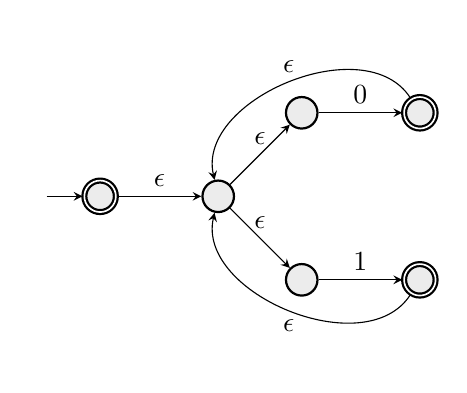
\begin{tikzpicture}[
                                styleSmall/.style={minimum size=4mm},
                                node distance=1.5cm,
                            ]
                            \node[state, accepting, initial, styleSmall] (q01asts) {};
                            \node[state, styleSmall, right of=q01asts] (q01sum) {};
                            \node[state, above right of=q01sum, styleSmall] (q01sum0) {};
                            \node[state, accepting, right of=q01sum0, styleSmall] (q01sum00) {};
                            \node[state, below right of=q01sum, styleSmall] (q01sum1) {};
                            \node[state, accepting, right of=q01sum1, styleSmall] (q01sum11) {};
                            \draw
                            (q01asts) edge[above] node{$\epsilon$} (q01sum)
                            (q01sum) edge[above] node{$\epsilon$} (q01sum0)
                            (q01sum) edge[above] node{$\epsilon$} (q01sum1)
                            (q01sum0) edge[above] node{$0$} (q01sum00)
                            (q01sum1) edge[above] node{$1$} (q01sum11)
                            (q01sum00) edge[bend right=80, above] node{$\epsilon$} (q01sum)
                            (q01sum11) edge[bend left=80, below] node{$\epsilon$} (q01sum);
                        \end{tikzpicture}
                        \caption{$(0 \cup 1)^\ast$}
                    \end{figure}
                    \begin{figure}[H]
                        \centering
                        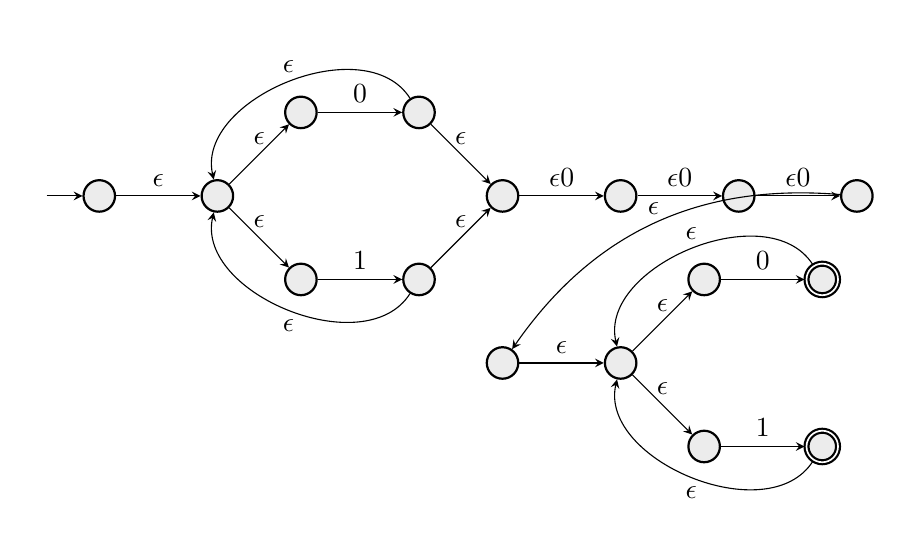
\begin{tikzpicture}[
                                styleSmall/.style={minimum size=4mm},
                                node distance=1.5cm,
                            ]
                            \node[state, initial, styleSmall] (q01asts) {};
                            \node[state, styleSmall, right of=q01asts] (q01sum) {};
                            \node[state, above right of=q01sum, styleSmall] (q01sum0) {};
                            \node[state, right of=q01sum0, styleSmall] (q01sum00) {};
                            \node[state, below right of=q01sum, styleSmall] (q01sum1) {};
                            \node[state, right of=q01sum1, styleSmall] (q01sum11) {};

                            \node[state, below right of=q01sum00, styleSmall] (qzs) {};
                            \node[state, right of=qzs, styleSmall] (qz0) {};
                            \node[state, right of=qz0, styleSmall] (qz00) {};
                            \node[state, right of=qz00, styleSmall] (qz000) {};

                            \node[state, below right of=q01sum11, styleSmall] (q21asts) {};
                            \node[state, styleSmall, right of=q21asts] (q21sum) {};
                            \node[state, above right of=q21sum, styleSmall] (q21sum0) {};
                            \node[state, accepting, right of=q21sum0, styleSmall] (q21sum00) {};
                            \node[state, below right of=q21sum, styleSmall] (q21sum1) {};
                            \node[state, accepting, right of=q21sum1, styleSmall] (q21sum11) {};
                            \draw
                            (q01asts) edge[above] node{$\epsilon$} (q01sum)
                            (q01sum) edge[above] node{$\epsilon$} (q01sum0)
                            (q01sum) edge[above] node{$\epsilon$} (q01sum1)
                            (q01sum0) edge[above] node{$0$} (q01sum00)
                            (q01sum1) edge[above] node{$1$} (q01sum11)
                            (q01sum00) edge[bend right=80, above] node{$\epsilon$} (q01sum)
                            (q01sum11) edge[bend left=80, below] node{$\epsilon$} (q01sum)

                            (q01sum00) edge[above] node{$\epsilon$} (qzs)
                            (q01sum11) edge[above] node{$\epsilon$} (qzs)

                            (qzs) edge[above] node{$\epsilon0$} (qz0)
                            (qz0) edge[above] node{$\epsilon0$} (qz00)
                            (qz00) edge[above] node{$\epsilon0$} (qz000)

                            (qz000) edge[above, bend right] node{$\epsilon$} (q21asts)

                            (q21asts) edge[above] node{$\epsilon$} (q21sum)
                            (q21sum) edge[above] node{$\epsilon$} (q21sum0)
                            (q21sum) edge[above] node{$\epsilon$} (q21sum1)
                            (q21sum0) edge[above] node{$0$} (q21sum00)
                            (q21sum1) edge[above] node{$1$} (q21sum11)
                            (q21sum00) edge[bend right=80, above] node{$\epsilon$} (q21sum)
                            (q21sum11) edge[bend left=80, below] node{$\epsilon$} (q21sum);
                        \end{tikzpicture}
                        \caption{$(0 \cup 1)^\ast000(0 \cup 1)^\ast$}
                    \end{figure}
              \item $(((00)^\ast(11)) \cup 01)^\ast$
                    \begin{figure}[H]
                        \centering
                        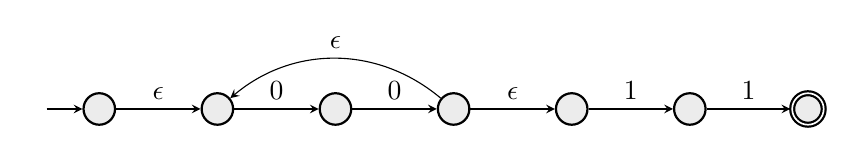
\begin{tikzpicture}[
                                styleSmall/.style={minimum size=4mm},
                                node distance=1.5cm,
                            ]
                            \node[state, initial, styleSmall] (q0e) {};
                            \node[state, styleSmall, right of=q0e] (q0) {};
                            \node[state, right of=q0, styleSmall] (q01) {};
                            \node[state, right of=q01, styleSmall] (q02) {};
                            \node[state, right of=q02, styleSmall] (q1e) {};
                            \node[state, right of=q1e, styleSmall] (q11) {};
                            \node[state, accepting, right of=q11, styleSmall] (q12) {};
                            \draw
                            (q0e) edge[above] node{$\epsilon$} (q0)
                            (q0) edge[above] node{$0$} (q01)
                            (q01) edge[above] node{$0$} (q02)
                            (q02) edge[bend right=40, above] node{$\epsilon$} (q0)
                            (q02) edge[above] node{$\epsilon$} (q1e)
                            (q1e) edge[above] node{$1$} (q11)
                            (q11) edge[above] node{$1$} (q12);
                        \end{tikzpicture}
                        \caption{$((00)^\ast(11))$}
                    \end{figure}
                    \begin{figure}[H]
                        \centering
                        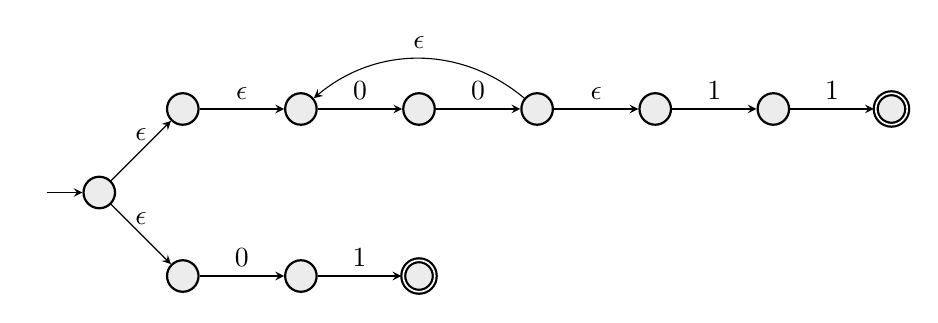
\begin{tikzpicture}[
                                styleSmall/.style={minimum size=4mm},
                                node distance=1.5cm,
                            ]
                            \node[state, initial, styleSmall] (qse) {};
                            \node[state, above right of=qse, styleSmall] (q0e) {};
                            \node[state, styleSmall, right of=q0e] (q0) {};
                            \node[state, right of=q0, styleSmall] (q01) {};
                            \node[state, right of=q01, styleSmall] (q02) {};
                            \node[state, right of=q02, styleSmall] (q1e) {};
                            \node[state, right of=q1e, styleSmall] (q11) {};
                            \node[state, accepting, right of=q11, styleSmall] (q12) {};
                            \node[state, below right of=qse, styleSmall] (qs1) {};
                            \node[state, right of=qs1, styleSmall] (qs2) {};
                            \node[state, accepting, right of=qs2, styleSmall] (qs3) {};
                            \draw
                            (q0e) edge[above] node{$\epsilon$} (q0)
                            (q0) edge[above] node{$0$} (q01)
                            (q01) edge[above] node{$0$} (q02)
                            (q02) edge[bend right=40, above] node{$\epsilon$} (q0)
                            (q02) edge[above] node{$\epsilon$} (q1e)
                            (q1e) edge[above] node{$1$} (q11)
                            (q11) edge[above] node{$1$} (q12)
                            (qse) edge[above] node{$\epsilon$} (q0e)
                            (qse) edge[above] node{$\epsilon$} (qs1)
                            (qs1) edge[above] node{$0$} (qs2)
                            (qs2) edge[above] node{$1$} (qs3);
                        \end{tikzpicture}
                        \caption{$((00)^\ast(11)) \cup 01$}
                    \end{figure}
                    \begin{figure}[H]
                        \centering
                        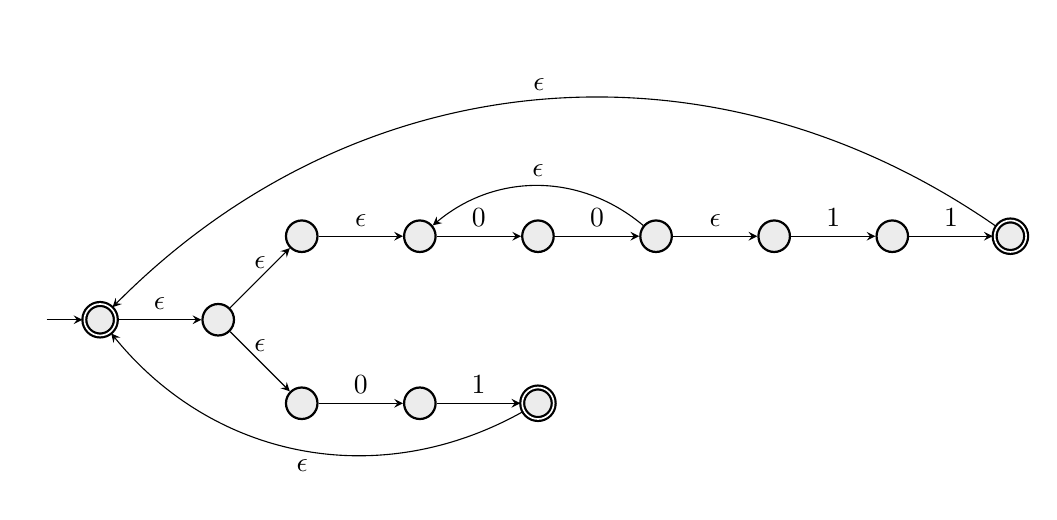
\begin{tikzpicture}[
                                styleSmall/.style={minimum size=4mm},
                                node distance=1.5cm,
                            ]
                            \node[state, initial, accepting, styleSmall] (q3e) {};
                            \node[state, styleSmall, right of=q3e] (qse) {};
                            \node[state, above right of=qse, styleSmall] (q0e) {};
                            \node[state, styleSmall, right of=q0e] (q0) {};
                            \node[state, right of=q0, styleSmall] (q01) {};
                            \node[state, right of=q01, styleSmall] (q02) {};
                            \node[state, right of=q02, styleSmall] (q1e) {};
                            \node[state, right of=q1e, styleSmall] (q11) {};
                            \node[state, accepting, right of=q11, styleSmall] (q12) {};
                            \node[state, below right of=qse, styleSmall] (qs1) {};
                            \node[state, right of=qs1, styleSmall] (qs2) {};
                            \node[state, accepting, right of=qs2, styleSmall] (qs3) {};
                            \draw
                            (q0e) edge[above] node{$\epsilon$} (q0)
                            (q0) edge[above] node{$0$} (q01)
                            (q01) edge[above] node{$0$} (q02)
                            (q02) edge[bend right=40, above] node{$\epsilon$} (q0)
                            (q02) edge[above] node{$\epsilon$} (q1e)
                            (q1e) edge[above] node{$1$} (q11)
                            (q11) edge[above] node{$1$} (q12)
                            (qse) edge[above] node{$\epsilon$} (q0e)
                            (qse) edge[above] node{$\epsilon$} (qs1)
                            (qs1) edge[above] node{$0$} (qs2)
                            (qs2) edge[above] node{$1$} (qs3)
                            (q3e) edge[above] node{$\epsilon$} (qse)
                            (q12) edge[bend right=40, above] node{$\epsilon$} (q3e)
                            (qs3) edge[bend left=40, below] node{$\epsilon$} (q3e);
                        \end{tikzpicture}
                        \caption{$(((00)^\ast(11)) \cup 01)^\ast$}
                    \end{figure}
              \item $\emptyset$
                    \begin{figure}[H]
                        \centering
                        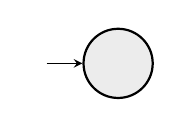
\begin{tikzpicture}
                            \node[state, initial] (q0) {};
                            \draw;
                        \end{tikzpicture}
                    \end{figure}
          \end{enumerate}

    \item [1.20]
          For each of the following languages, give two strings that are members and two strings that are not members—a total of four strings for each part. Assume the alphabet $\Sigma=\{a,b\}$ in all parts.
          \begin{enumerate}
              \item $a^\ast b^\ast $
                    \begin{table}[H]
                        \centering
                        \begin{tabular}{|c|c|}
                            \hline
                            Members    & Not Members \\
                            \hline
                            $\epsilon$ & $bbba$      \\
                            $ab$       & $abab$      \\
                            \hline
                        \end{tabular}
                    \end{table}
              \item $a(ba)^\ast b $
                    \begin{table}[H]
                        \centering
                        \begin{tabular}{|c|c|}
                            \hline
                            Members    & Not Members \\
                            \hline
                            $ab$       & $b$         \\
                            $aabababb$ & $aaab$      \\
                            \hline
                        \end{tabular}
                    \end{table}
              \item $a^\ast \cup b^\ast $
                    \begin{table}[H]
                        \centering
                        \begin{tabular}{|c|c|}
                            \hline
                            Members & Not Members \\
                            \hline
                            $aaa$   & $ab$        \\
                            $bbbb$  & $baba$      \\
                            \hline
                        \end{tabular}
                    \end{table}
              \item $(aaa)^\ast $
                    \begin{table}[H]
                        \centering
                        \begin{tabular}{|c|c|}
                            \hline
                            Members    & Not Members \\
                            \hline
                            $\epsilon$ & $b$         \\
                            $aaaaaa$   & $aa$        \\
                            \hline
                        \end{tabular}
                    \end{table}
              \item $\Sigma^\ast a\Sigma^\ast b\Sigma^\ast a\Sigma^\ast $
                    \begin{table}[H]
                        \centering
                        \begin{tabular}{|c|c|}
                            \hline
                            Members   & Not Members \\
                            \hline
                            $aba$     & $aaaa$      \\
                            $ababbbb$ & $bb$        \\
                            \hline
                        \end{tabular}
                    \end{table}
              \item $aba \cup bab $
                    \begin{table}[H]
                        \centering
                        \begin{tabular}{|c|c|}
                            \hline
                            Members & Not Members \\
                            \hline
                            $aba$   & $ababab$    \\
                            $bab$   & $abb$       \\
                            \hline
                        \end{tabular}
                    \end{table}
              \item $ (\epsilon  \cup a)b $
                    \begin{table}[H]
                        \centering
                        \begin{tabular}{|c|c|}
                            \hline
                            Members & Not Members \\
                            \hline
                            $b$     & $\epsilon$  \\
                            $ab$    & $aaba$      \\
                            \hline
                        \end{tabular}
                    \end{table}
              \item $(a\cup ba \cup bb)\Sigma$
                    \begin{table}[H]
                        \centering
                        \begin{tabular}{|c|c|}
                            \hline
                            Members & Not Members \\
                            \hline
                            $aa$    & $bbaa$      \\
                            $bbb$   & $abb$       \\
                            \hline
                        \end{tabular}
                    \end{table}
          \end{enumerate}

    \item [1.21]

          Use the procedure described in Lemma 1.60 to convert the following finite automata to regular expressions.
          \begin{enumerate}
              \item

                    \begin{figure}[H]
                        \centering
                        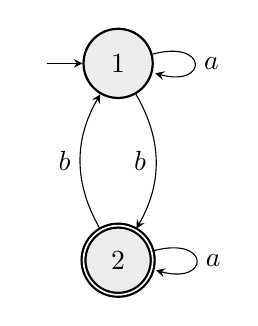
\begin{tikzpicture}
                            \node[state, initial] (q1) {1};
                            \node[state, below of=q1, accepting] (q2) {2};
                            \draw
                            (q1) edge[bend left, left] node{$b$} (q2)
                            (q2) edge[bend left, left] node{$b$} (q1)
                            (q1) edge[loop right] node{$a$} (q1)
                            (q2) edge[loop right] node{$a$} (q2)
                            ;
                        \end{tikzpicture}
                    \end{figure}

                    $b(a)^\ast b \cup a^\ast$
                    
              \item

                    \begin{figure}[H]
                        \centering
                        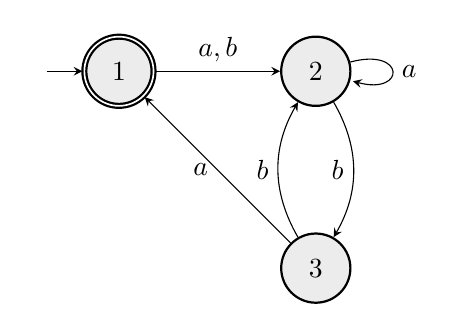
\begin{tikzpicture}
                            \node[state, initial, accepting] (q0) {1};
                            \node[state, right of=q0] (q1) {2};
                            \node[state, below of=q1] (q2) {3};;
                            \draw
                            (q1) edge[bend left, left] node{$b$} (q2)
                            (q2) edge[bend left, left] node{$b$} (q1)
                            (q2) edge[left, left] node{$a$} (q0)
                            (q0) edge[left, above] node{$a,b$} (q1)
                            (q1) edge[loop right] node{$a$} (q1)
                            ;
                        \end{tikzpicture}
                    \end{figure}

                    $a(a^\ast \cup bb)a \cup b(a^\ast \cup bb)a $
          \end{enumerate}
\end{enumerate}

\end{document}
